\documentclass{article}
\usepackage{amsmath,amssymb,graphicx,tikz}
\usepackage{hyperref}
\usepackage{tikz}
\usepackage{amsfonts}
\usepackage{amsmath}
\usepackage{listings}

\title{CSC263 Winter 2016, Assignment 2}
\author{Connor Peet \#1001088208}
\renewcommand{\today}{~}
\hypersetup{pdfpagemode=Fullscreen,
  colorlinks=true,
  linkfileprefix={}}
\begin{document}
\maketitle

\lstset{
    numbers=left
}

\begin{enumerate}
\item [1.] See figures 1 and 2 on the following page.
    \begin{figure}[p]
    \centering
    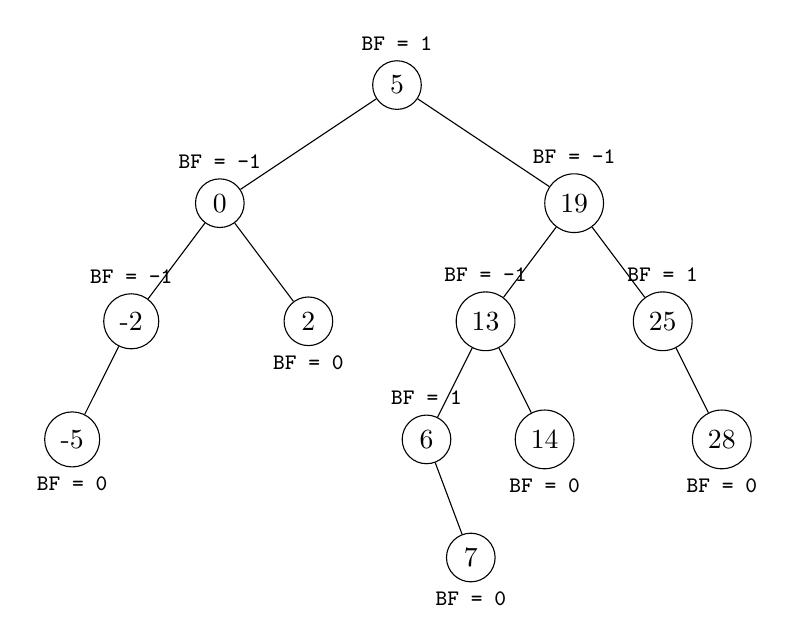
\begin{tikzpicture}[
        level/.style={sibling distance=45mm/#1, level distance = 15mm},
        every node/.style={align=center},
        label distance=0mm,
        every label/.style={text width=20mm, below},
    ]
    \tikzstyle{every label}=[font=\footnotesize]
    \node[circle,draw,label=\texttt{BF = 1}]{5}
        child{ node[circle,draw, label=\texttt{BF = -1}]{0}
            child{ node[circle,draw,label=\texttt{BF = -1}]{-2}
                child{ node[circle,draw,label=below:\texttt{BF = 0}]{-5} }
                child[missing]{}
            }
            child{ node[circle,draw,label=below:\texttt{BF = 0}]{2} }
        }
        child{ node[circle,draw,label=\texttt{BF = -1}]{19}
            child{ node[circle,draw,label=\texttt{BF = -1}]{13}
                child{ node[circle,draw,label=\texttt{BF = 1}]{6}
                    child[missing]{}
                    child{ node[circle,draw,label=below:\texttt{BF = 0}]{7} }
                }
                child{ node[circle,draw,label=below:\texttt{BF = 0}]{14} }
            }
            child{ node[circle,draw,label=\texttt{BF = 1}]{25}
                child[missing]{}
                child{ node[circle,draw,label=below:\texttt{BF = 0}]{28} }
            }
        };
    \end{tikzpicture}
    \caption{The resulting AVL tree $T$.}
    \end{figure}

    \begin{figure}[p]
    \centering
    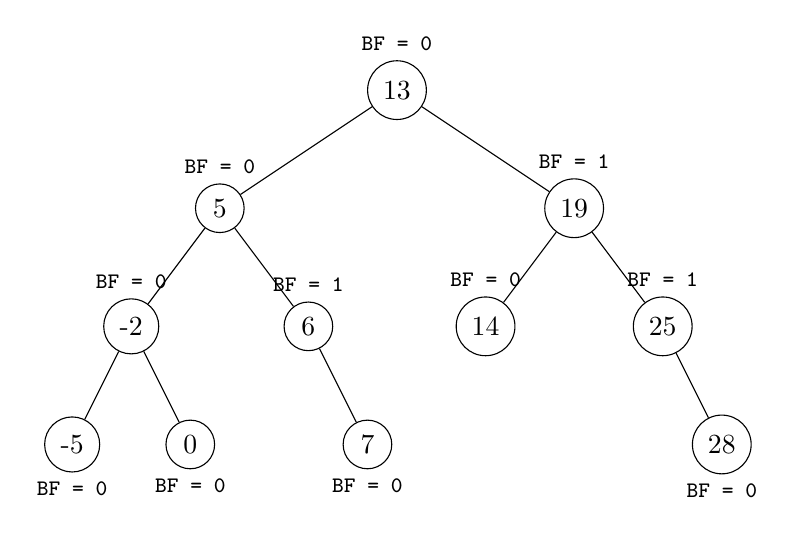
\begin{tikzpicture}[
        level/.style={sibling distance=45mm/#1, level distance = 15mm},
        every node/.style={align=center},
        label distance=0mm,
        every label/.style={text width=20mm, below},
    ]
    \tikzstyle{every label}=[font=\footnotesize]
    \node[circle,draw,label=\texttt{BF = 0}]{13}
        child{ node[circle,draw, label=\texttt{BF = 0}]{5}
            child{ node[circle,draw,label=\texttt{BF = 0}]{-2}
                child{ node[circle,draw,label=below:\texttt{BF = 0}]{-5} }
                child{ node[circle,draw,label=below:\texttt{BF = 0}]{0} }
            }
            child{ node[circle,draw,label=\texttt{BF = 1}]{6}
                child[missing]{}
                child{ node[circle,draw,label=below:\texttt{BF = 0}]{7} }
            }
        }
        child{ node[circle,draw,label=\texttt{BF = 1}]{19}
            child{ node[circle,draw,label=\texttt{BF = 0}]{14} }
            child{ node[circle,draw,label=\texttt{BF = 1}]{25}
                child[missing]{}
                child{ node[circle,draw,label=below:\texttt{BF = 0}]{28} }
            }
        };
    \end{tikzpicture}
    \caption{$T$ after deleting $2$ and executing the necessary rotations.}
    \end{figure}

\item [2.] First we define a \texttt{pull\_root} function that takes removes and returns either the smallest element of $B_2$ or the largest element of $B_1$.
\begin{lstlisting}
def pull_root(B1, B2):
    node_b1 = B1.root
    node_b2 = B2.root

    while True:
        if node_b1.right == nil:
            if node_b1.parent != nil:
                node_b1.parent.right = nil
            return node_b1

        elif node_b2.left == nil:
            if node_b2.parent != nil:
                node_b2.parent.left = nil
            return node_b2

        node_b1 = node_b1.right
        node_b2 = node_b2.left
\end{lstlisting}

    The function to merge the trees is a trivial extension of \texttt{pull\_root}:
\begin{lstlisting}
def merge(B1, B2):
    root = pull_root(B1, B2)
    root.left = B1
    root.right = B2
    B1.parent = root
    B2.parent = root
\end{lstlisting}

    In this function, we're running down the right-most subtrees of $B_1$ and left-most subtrees of $B_2$ until we get to the leaf of either. This relies on the invariants of BSTs. When the node is found, it's removed from its parent and returned. The while loop will run at most $min\{h_1, h_2\}$ times--it loops down $B_1$ and $B_2$ and aborts as soon as it reaches a leaf of either--and each function inside the loop takes a constant time, so the function is in $O(min\{h_1, h_2\})$. \\

    The leaf that's removed and returned is either the largest item in $B_1$ or the smallest item in $B_2$. In both cases this item can be assigned to the root of the tree while preserving the BST property. \\

    The maximum height change occurs when the removed leaf was not the single deepest node out of both trees. When this occurs, the height of the new tree $T$ is $max\{h_1, h_2\} + 1$ as the result of inserting a new root above the subtrees. If this is not the case, then height of $T$ will equal $max\{h_1, h_2\}$.

\end{enumerate}
\end{document}
